\documentclass[11pt,a4paper]{article}
\usepackage{polski}
\usepackage[utf8]{inputenc} 

\usepackage{graphicx}



\title{Laboratorium 6 - Sprawozdanie}
\author{Wojciech Makuch}

\begin{document}
\maketitle
\section{Zadanie}
Poprawa programu framework benchmarkujacy dla algorytmu sortowania szybkiego na strukturze kolejka utworzonym na liscie bazując na kodzie uzytkownika Sheaim/209226. Zadanie polegało na optymalizacji algorytmu i porównania złożoności obliczeniowej.
\section{Realizacja}
Na samym początku zwrócono uwagę na niepoprawne działanie listy. Usunieto ten problem modyfikując metody \textsl{delete\_cell(int)}, \textsl{add(cell*,int)}, \textsl{Zamien(int,int)}. Lista działa poprawnie z indeksowaniem od 1 elementu(dla sortrowania nie stanowi to problemu, zerowy element wypełniono zerem :-). Program wzbogacono o metody sortowania szybkiego, które za piwota wybierają: pierwszy element, medianę z losowego ciągu trzech liczb oraz środkowy element. Ponadto podzielono program na moduły z rozszeżeniami \textsl{.hh} oraz \textsl{.cpp}. Do programu nie utworzono dokumentacji, ponieważ kod źródłowy należy do innego użytkownika.



\section{Działanie}
Program nie udostępnia menu użytkownika. Główna funkcja programu wywołuje jedynie funkcję benchmarkującą, która zawiera pętle zliczającą czas trwania sortowania szybkeigo, wyswietlając dane na strumień wyjściowy i zapisując do pliku o nazwie \textsl{pomiar\_czasu\_6.txt}. Program zlicza czas dla trzech metod pokoleji: piwot - skrajny element, piwot - mediana oraz piwot - środkowy element.

\section{Wyniki}
Na rys 1. pokazano wykresy złożoności obliczeniowej dla wymienionych metod sortowania szybkiego. Ponadto zamieszczono dla porównania wykres funkcji liniowej oraz funkcji $n log n$. 

\begin{figure}
\centering
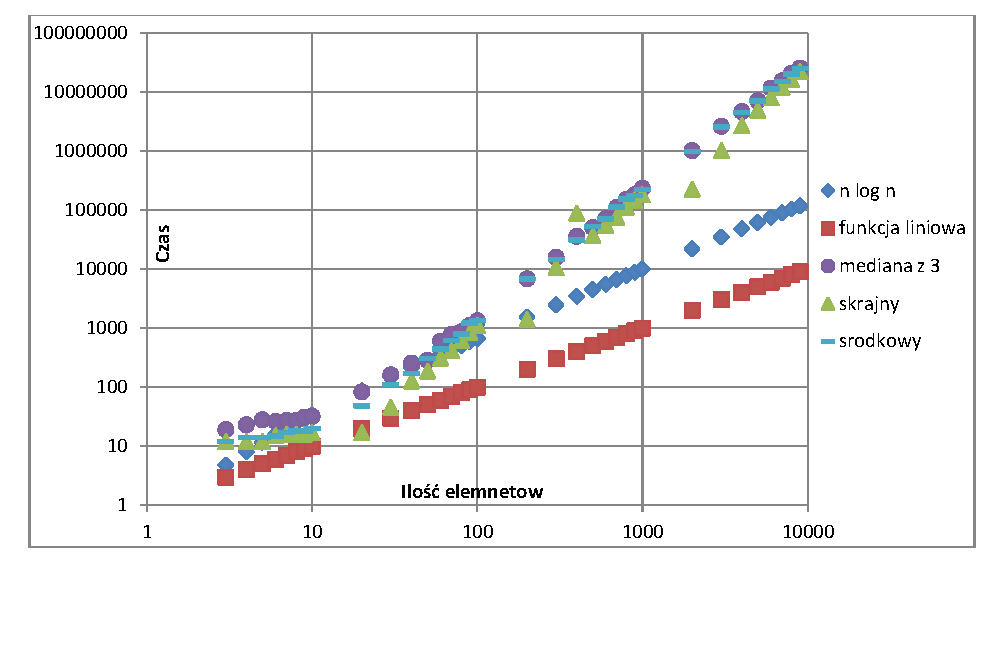
\includegraphics[scale=0.75]{wykr.pdf}
\caption{Wykres złożoności obliczeniowej dla dużej ilości elementów.}
\label{fig:wykres1}
\end{figure}



\section{Wnioski}
\begin{enumerate}
\item Wszystkie metody sortowania dla duzej ilości elementów degenerują się do $O(n^{2}).$
\item Do 100 elementów przebiegi sortowań pokrywają sie z przebiegiem $n log n.$
\item Dla piwota wyliczonego jako mediana z trzech liczb losowego ciągu oraz dla piwota środkowego wykresy pokrywają się już dla ilości większej od 50.
\item Wykres dla złożoności - piwot - skrajny element styka się z przebiegiem liniowym dla bardzo małych wartości. Ponadto dla dużych ilości elementów degeneruje się najwolniej.
\end{enumerate}

\section{Podsumowane}
Średnia złozoność obliczeniowa algorymtu sortowania szybkiego wynosi $O(nlogn)$. W przypadku pesymistycznym oraz dla dużych ilości elementów do posortowania złożoność degeneruje się do $O(n^{2})$.


\section{Komentarz}
Do utworzenia dokumentacji wykorzystano system Doxygen.
Funkcja pomiaru czasu dla systemu Windows pobrana ze strony dr. J. Mierzwy. Program skompilowano w środowisku Code::Blocks. Do stworzonia wykresu posłużono się pakietem MS Excel, sprawozdanie napisano używając systemu \LaTeX.
\end{document}